\chapter{Sommaire (en Français)}
\label{chapter:sommaire}
\pagestyle{mainmatter}
\pagenumbering{arabic}

Comprendre le cerveau humain  est l'un des défis les plus importants du 21e siècle. Sans doute l'organe le plus complexe du corps humain, le cerveau est responsable  d’un large éventail de fonctions cognitives telles la reconnaissance visuelle, la compréhension du langage, la production de la parole, les interactions sociales et le contrôle exécutif. Les pathologies associées au cerveau demeurent, à ce jour, une problématique extrêmement complexe.  Actuellement, les interventions médicales pour les principales maladies infectieuses permettent aux individus de vivre jusqu'à l’âge de 80 et même  90 ans. Malgré les avancées de la médecine, nous n’arrivons pas à cibler efficacement les mécanismes  qui engendrent ou qui contribuent à la progression des pathologies mentales, telles le Parkinson, la démence d’Alzheimer, la schizophrénie  et l’épilepsie, pour n'en nommer que quelques-unes. Ceci a de graves conséquences sur la société vieillissante, par exemple une personne  dans la quarantaine a 50\% de risque de développer la maladie d'Alzheimer ~\citep{alzheimer20162016}.

Néanmoins, notre compréhension actuelle du cerveau est le résultat de décennies d'efforts concertés dans de multiples disciplines allant de la biologie moléculaire, à la génétique et la physiologie, en passant par les neurosciences cognitives et comportementales, la statistique, l'informatique et la science des données. Un sous-domaine en expansion est l'imagerie cérébrale, également connue sous le nom de neuroimagerie. L'imagerie cérébrale fait référence à un ensemble de technologies où l'on mesure l’activité  instantanée du cerveau. Ces mesures peuvent être statiques, comme dans le cas des images anatomiques issues de l'imagerie par résonance magnétique (IRM), ou dynamique, comme dans le cas de l'imagerie par résonance magnétique fonctionnelle (IRMf). L’objectif à long-terme serait d’utiliser ces techniques  dans les hôpitaux pour aider au niveau du diagnostic et dans les chirurgies, dans les interface neuronale directe (IND) et dans la recherche en neurosciences. Cette thèse sera dédiée à  la mesure des courants électriques et/ou du champ magnétique du cerveau par l’entremise de l'électroencéphalographie (EEG), de la magnétoencéphalographie et les potentiels de champ local (LFP). Ces méthodes ont la propriété de posséder une résolution temporelle élevée,ce qui est particulièrement utile pour extraire la dynamique temporelle des signaux du cerveau.

Dans cette thèse, j’élabore sur l’optimisation des analyses  de données publiques en  neuroimagerie , et ce, au moyen des logiciels libres. À cet effet, j'ai participé à une collaboration internationale pour créer une norme sur les analyses en MEG pour la structure de données d'imagerie cérébrale (BIDS)~\citep{niso2018meg}. J'ai écrit le validateur qui a aidé à créer les exemples d'ensembles de données compatibles MEG-BIDS. En tant que collaborateur de MNE~\citep{gramfort2013meg}, j'ai dirigé la rédaction d'un tutoriel qui permet d’analyser à nouveau un ensemble de données, nommé Faces~\citep{wakeman2015multi}, pour une reproduire les résultats préalablement retrouvés.Dans le contexte du mouvement de reproductibilité et de partage des données, nous avons commencé à automatiser nos séquences d’étapes d’analyses (pipelines), ce qui nous a amené à développer un algorithme entièrement automatisé pour le rejet et la réparation des artefacts en EEG/MEG~\citep{jas2016automated, jas2017autoreject}. Enfin, nous avons développé des algorithmes pour permettre l’apprentissage automatique de nouveaux motifs (patterns) cérébraux qui n’ont pas pu être démontré  par l’utilisation de données extraites de séries temporelles neuronales~\citep{jas2017learning}. 

La thèse est organisée par chapitres pour mettre en évidence ces quatre principaux domaines de contribution : le partage des données, la reproductibilité, l'automatisation de la détection des artefacts et la découverte automatisée des motifs cérébraux à partir des données EEG/MEG. Un aspect important de cette thèse est que ces contributions ont conduit non seulement à des publications dans des conférences et revues internationales, mais aussi à des implémentations open source reproductibles et à des ensembles de données réutilisables. Une liste complète est donnée ci-dessous.

\subsection*{Publications dans les revues}
\bibentry{jas2017autoreject}\ \\ \\
\bibentry{jas2017mne}\ \\ (Pending revision at \emph{Frontiers in Neuroscience, Brain Imaging Methods})\ \\ \\
\bibentry{niso2018meg}

\subsection*{Publications dans les conférences}
\bibentry{jas2016automated}\ \\ \\
\bibentry{jas2017learning}

\subsection*{Documents d'atelier}
\bibentry{dengemann2015conc}\

\subsection*{Implémentations Open Source}

\url{http://autoreject.github.io/} \\
\url{http://alphacsc.github.io/} \\
\url{http://mne-tools.github.io/mne-biomag-group-demo/}\\
\url{https://jasmainak.github.io/bids-validator/}

\subsection*{Datasets}

\url{https://openfmri.org/dataset/ds000248/}

Dans le résumé en français, je présenterai le contexte de la thèse, suivi d'un bref résumé de chacun des quatre principaux domaines de contribution.

\section*{Électrophysiologie}

\begin{figure}[htb]
\begin{center}
   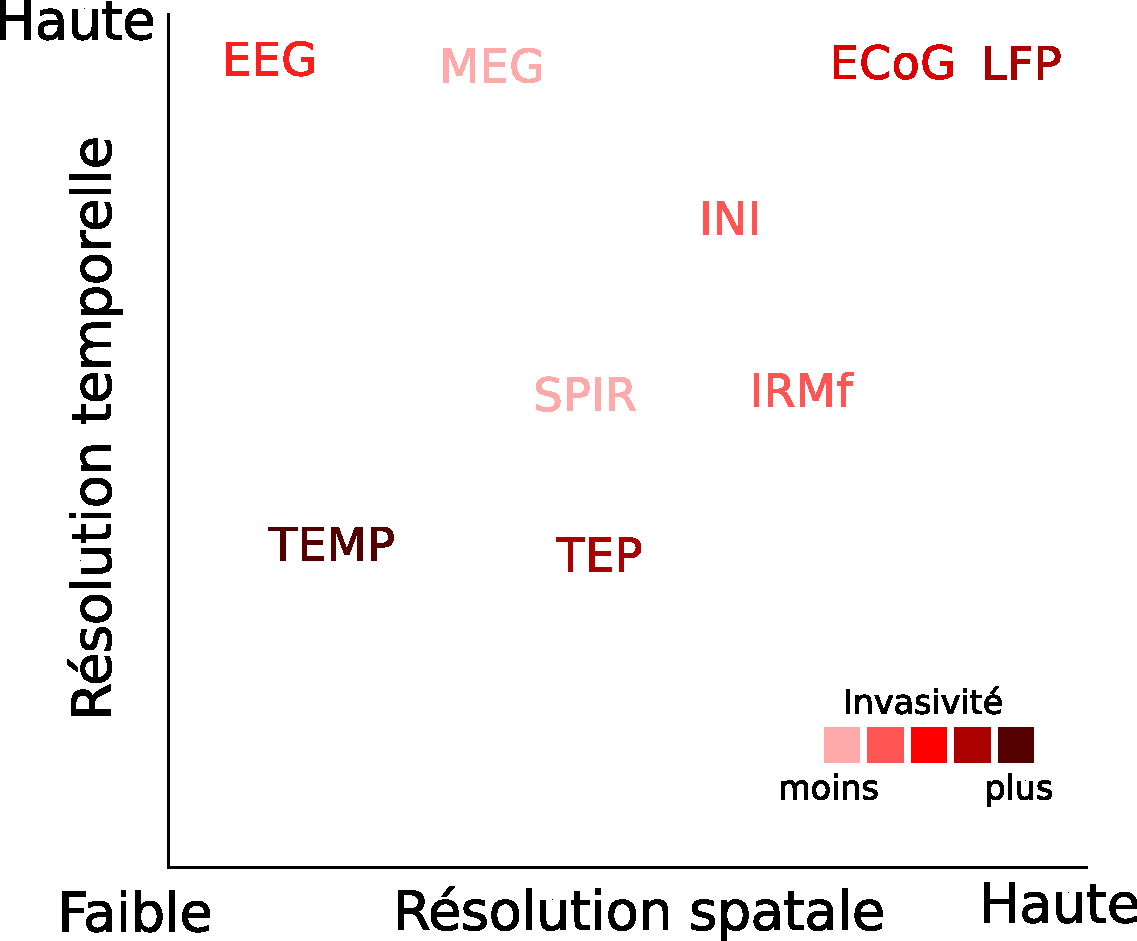
\includegraphics[width=0.6\linewidth]{figures/neuroimaging_methods_sommaire.pdf}
\end{center}
   \caption[]{Diverses méthodes de neuroimagerie diffèrent en termes d'information qu'elles mesurent. MEG=magnétoencéphalographie, EEG=électroencéphalographie, SPIR=spectroscopie par proche infrarouge, TEP=tomographie par émission de positons, TEMP=tomographie par émission de photons simples, et INI=imagerie inverse, une méthode pour accélérer l'acquisition d'images IRMf, ECoG=Electrocorticographie, LFP=Local Field Potential.}
   \label{fig:sommaire:neuroimaging_methods}
\end{figure}

Dans cette thèse, nous discuterons des données enregistrées principalement à l'aide de la MEG et de l’EEG. L'EEG et la MEG sont des méthodes d'électrophysiologie permettant d’étudier les propriétés des cellules et tissus biologiques. Les tissus biologiques ont des propriétés électriques dues à la présence d'ions. Tout comme nous pouvons mesurer les tensions dans les appareils électriques, il est également possible de mesurer ces tensions dans les tissus vivants.

L'enregistrement électrophysiologique a l'avantage de mesurer directement l'activité cérébrale, par opposition à une mesure indirecte, ce qui est par exemple le cas de l'IRMf. Les techniques d'imagerie cérébrale se caractérisent par leur résolution temporelle et spatiale, c'est-à-dire l'échelle de temps à laquelle elle peut mesurer l'activité cérébrale, ainsi que la précision de la localisation de la source de l'activité, respectivement. La Figure~\ref{fig:sommaire:neuroimaging_methods} résume les différentes méthodes de neuroimagerie en ce qui concerne leur résolution temporelle et spatiale, mais aussi leur caractère invasif. Ceci est utile pour comprendre pourquoi la MEG/EEG est souvent considéré comme la méthode de choix pour comprendre les fondements de l'activité cérébrale humaine. Bien que l'IRMf soit une autre méthode non invasive, elle mesure le flux sanguin qui est une réponse lente en comparaison à l'activité neuronale ce qui lui confère une résolution temporelle peut élevée.

Il existe un certain nombre de méthodes pour mesurer les potentiels électriques dans le corps humain, la plus connue étant peut-être l'électrocardiographie (ECG) qui est utilisée pour mesurer l'activité électrique du cœur. Les trois méthodes dont nous discutons dans la thèse produisent des séries temporelles multivariées. Un bref résumé de chacune de ces méthodes est présenté ci-dessous.

\paragraph{Électroencéphalographie :} L'EEG est une technique de mesure portable et non invasive inventée dans les années 1920 et utilisée dans plusieurs contextes tels que les IND, la surveillance médicale et dans l’établissement de diagnostic, ainsi que dans les études cognitives. En électroencéphalographie, un réseau d'électrodes sur un capuchon d’EEG est placé sur le cuir chevelu pour mesurer les tensions par rapport à une électrode de référence. La tension qu'il mesure n'est pas  la résultante d'un seul neurone, mais plutôt le résultat de l'activité électrique de populations de neurones lui conférant une résolution temporelle élevée (de l'ordre des \emph{ms}), quoique la résolution spatiale n'est pas si élevée.

\paragraph{Magnétoencéphalographie :} Tout courant électrique est associé à des champs magnétiques en fonction de la théorie de Maxwell. En effet, le cerveau génère de minuscules champs magnétiques qui s'enroulent autour des courants électriques selon la règle de la main droit de Maxwell. Le champ magnétique du cerveau est minuscule ($\sim10^{-12}T$) comparé au champ magnétique terrestre ($\sim10^{-4}T$) et au bruit magnétique ambiant ($\sim10^{-6}T$). . Par conséquent, pour le mesurer, on a besoin d'une mesure électronique très sensible et d'une annulation de bruit important. La mesure elle-même se fait dans une salle blindée magnétiquement, composée de trois couches de métaux. Les capteurs sont des bobines supraconductrices qui capturent le flux magnétique. Ils sont immergés dans de l'hélium liquide à de très basses températures (autour de 4 K), afin de réduire toute perte de signal due à la résistance. Un appareil typique contient deux types de capteurs : les gradiomètres et les magnétomètres. Tandis que le magnétomètre mesure l'amplitude absolue du champ magnétique, le gradiomètre mesure le gradient du champ. La MEG a l'avantage que le crâne ne détériore pas la qualité du signal contrairement à l'EEG.

\paragraph{Potentiel de champ local (LFP) :}
Le potentiel de champ local est le potentiel électrique qui est enregistré dans l'espace extracellulaire du tissu cérébral. Contrairement à l'EEG, les LFP sont enregistrés en profondeur, à partir du tissu cortical et peuvent donc mesurer des populations de neurones plus localisées. De petites électrodes intracrâniennes sont généralement utilisées pour mesurer ces potentiels, contrairement aux électrodes de grande surface utilisées dans l'EEG.

\section*{Contexte de la thèse}
La thèse se focalise sur les récents mouvements de reproductibilité et de partage des données en neuroimagerie. Elle met l'accent sur la simplification de l'analyse des données grâce à de meilleurs outils pédagogiques et à des méthodes automatisées permettant une analyse reproductible à l'ère des grandes données.

\subsection*{La crise de la reproductibilité}
\label{sec:sommaire:reproducibility_crisis}
Même si des milliers d'articles sont publiés à chaque année sur différents aspects du cerveau, notre compréhension de cet organe complexe n'est pas proportionnelle. Une grande partie de la raison a été attribuée à ce que l'on appelle la crise de la reproductibilité~\citep{ioannidis2005most, simmons2011false, button2013power}.
Les progrès de la science reposent sur des expériences reproductibles. La reproductibilité fait référence au fait que les résultats d'une expérience peuvent être régénérés, et ce, de manière indépendante,si le code, les données et les logiciels connexes ont été fournis. Dans de nombreux domaines, cependant, une grande partie des expériences ne peut être reproduite. En psychologie, par exemple, on a estimé que plus de la moitié des articles n'étaient pas reproductibles~\citep{open2015estimating}, et même ceux qui pouvaient être reproduits avaient tendance à avoir un effet plus faible par rapport aux études originales.

Les raisons pour lesquelles les résultats ne sont pas reproductibles peuvent être nombreuses~\citep{baker20161}, certaines étant : 1) le biais de confirmation, la tendance à ne rapporter sélectivement que les expériences conformes aux croyances préexistantes du chercheur, 2) le ``p-hacking''~\citep{simmons2011false}, ou la tendance à essayer de multiples hypothèses pour obtenir un résultat positif, 3) le biais de publication ou l'absence d'incitation à publier des résultats négatifs~\citep{rosenthal1979file}, 4 ) corriger pour les comparaisons multiples, la méthode la plus conservatrice étant la correction de Bonferroni~\citep{dunn1961multiple} et 5) la pression à publier. Il existe maintenant un ensemble de recommandations acceptées pour régler bon nombre de ces questions. 

L'imagerie cérébrale a ses propres problèmes qui peuvent être liés à la crise de la reproductibilité :

% vul2009puzzlingly
% yendiki2014spurious

\begin{itemize}[noitemsep,partopsep=0pt]
\item \textbf{Manque de puissance statistique:} C'est sans doute l'une des questions centrales de la crise de la reproductibilité d'aujourd'hui et c'est de loin celle qui a reçu le plus d'attention. La puissance statistique d'une étude fait référence à la probabilité de découvrir un effet intéressant, compte tenu de la taille de l'échantillon. Les petites tailles d'échantillons se traduisent par des études sous-exploitées, ce qui signifie que le risque d'une fausse découverte est élevée. Afin de découvrir l'effet d'intérêt, l'étude doit être menée de façon appropriée.

%
\item \textbf{Comparaisons multiples:} Il s'agit essentiellement d'une manifestation de "piratage" qui résulte du grand nombre de voxels ou de points dans le temps en neuroimagerie. Par exemple, dans la célèbre étude sur le saumon mort~\citep{bennett2009neural}, un effet significatif a été trouvé même si aucun effet n'était attendu simplement parce que les tests d'hypothèse (comparaisons) ont été effectués sur chaque voxel.
%
\item \textbf{Différences dans les versions des logiciels :} Les changements de versions d’un logiciel peut conduire à des résultats différents. Par exemple, dans le cas du logiciel Freesurfer, les différences de volume étaient de l'ordre de $8.8\% \pm 6.6\%$ pour des versions différentes~\citep{gronenschild2012effects}.
%
\item \textbf{Pipelines complexes :} Les pipelines de neuroimagerie impliquent un certain nombre de choix à chaque étape de traitement, et il n'existe actuellement aucun consensus sur la façon de choisir les bonnes étapes d’analyses. Souvent, ces choix méthodologiques ne sont même pas documentés. On estime qu'il y a presque autant de pipelines uniques que d'études~\citep{Carp2012289}.
\item \textbf{Facteurs confusionnels:} Il existe plusieurs facteurs confusionnels tels que les mouvements de la tête~\citep{yendiki2014spurious}, les différences anatomiques et les changements dans la fréquence et la profondeur de la respiration, qui peuvent conduire à des corrélations fallacieuses.
\end{itemize}

Dans le Chapitre~\ref{chapter:group_study} de la thèse, nous fournirons des lignes directrices concrètes sur la façon de construire des pipelines de traitement des données MEG/EEG. Notre contribution abordera la question des pipelines complexes, des comparaisons multiples et des différences de versions de logiciels dans le cadre de la  MEG/EEG. La question de la puissance statistique peut être resolue par le partage des données, ce que nous allons aborder  dans la prochaine section.

\subsection*{Partage de données}
\label{sec:sommaire:intro_datasharing}
Le manque de puissance statistique est essentiellement dûe à la taille d’échantillon. Aujourd’hui, dans un environnement scientifique collaboratif et axé sur les données, le partage de données est utile non seulement du point de vue de la reproductibilité, mais aussi pour construire des ensembles de données avec des échantillons de grande taille. Avec de grands ensembles de données, il serait possible de distinguer même les effets subtils~\citep{smith2017statistical} qui n'étaient pas possibles avec de plus petits ensembles. Le partage de données est bénéfique non seulement du point de vue de la réplication, mais aussi d'un point de vue économique. Plutôt que de recueillir de nouvelles données pour chaque nouvelle hypothèse, les chercheurs peuvent maintenant ré-utiliser les données connues pour vérifier et valider leurs hypothèses.

Les avantages du partage de données remontent à Newton et à sa théorie de la gravitation~\citep{pointofview2013}. Avant que Newton ait développé sa théorie, un autre astronome anglais, John Flamsteed avait été nommé par le roi pour observer les étoiles et produire des cartes précises pour la navigation dans les mers. Sur une période de 40 ans, Flamsteed a créé un catalogue détaillé qui a triplé le nombre d'entrées dans l'atlas du ciel utilisé précédemment. Lorsque la grande comète de 1680 est apparue deux fois de suite dans le ciel, Flamsteed a utilisé ses données pour suggérer que ce n'était pas deux comètes mais bien la même comète qui s'est d'abord dirigée vers le soleil et s'en est ensuite détournée. Newton s'est d'abord opposé à cette théorie, mais il a changé d'avis plus tard en accédant au catalogue inédit de Flamsteed. La comète s'était en effet avérée être une référence importante pour la théorie de la gravitation de Newton.

Il est difficile d'imaginer à notre époque qu'une théorie aussi fondamentale que les lois de la gravitation aurait pu être guidée par les données. Le partage de données est fondamental non seulement pour la reproductibilité scientifique, mais il constitue également la base de l'apprentissage de modèles plus solides et de l'analyse comparative de nouveaux algorithmes. Par conséquent, dans le domaine de l'apprentissage automatique, les percées récentes ont été alimentées par l'augmentation du partage de données et du calcul. Cela inclut la croissance récente de l'apprentissage profond~\citep{deng2009imagenet}, l'apprentissage Q~\citep{watkins1992q, bellemare2013arcade}, le traitement du langage naturel pour la traduction du langage~\citep{halevy2009unreasonable}, la reconnaissance vocale~\citep{paul1992design}, et même le modèle du mélange d'experts~\citep{jacobs1991adaptive} pour IBM Watson~\citep{ferrucci2010building}. La maxime ``plus de données battent un algorithme plus intelligent''~\citep{domingos2012few} a remarquablement bien résisté à travers les disciplines et les âges.

Bien sûr, les neuroscientifiques commencent à prendre conscience de l'importance du partage de données. Récemment, les données neuronales ont commencé à être partagées par le biais de consortiums internationaux~\citep{van2013wu, ollier2005uk}, de dépôts de données~\citep{poldrack2013toward, gorgolewski2015neurovault} et d'articles sur les ensembles de données dans des revues ciblées. Pourtant, il y a encore un gros écart entre  l'idéal du partage de données et ce qui est pratiqué. Les expériences de neuroimagerie sont souvent très compliquées et il ne suffit pas de partager simplement les données, mais aussi les métadonnées et les informations concernant les protocoles expérimentaux dans un format bien structuré. En l'absence de cette information, les données partagées ne sont pas réutilisables de la même manière que les programmes peu commenté, mal structurés, et compliqués ne sont pas utiles même s'ils sont partagés publiquement. Il n'y a pas de consensus accepté au sein de la communauté sur les pratiques de partage des données et il est nécessaire d'établir une norme.
Au Chapitre~\ref{chapter:group_study}, nous présenterons une nouvelle norme connue sous le nom de BIDS, qui vise à combler cet écart. Il s'agit d'un effort de collaboration entre les développeurs de logiciels et les neuroscientifiques de divers laboratoires afin d'établir un consensus sur les normes et d'élaborer des outils pour faciliter l'adoption de la norme.

\subsection*{Automatisation}
\label{sec:sommaire:automation}

En 2014, Nature a publié un article audacieux~\citep{hayden2014automated} qui décrivait une vision de l'avenir de la science : des laboratoires automatisés qui enregistrerait de façon autonome chaque détail d'une expérience, ce qui mènerait à une recherche moins coûteuse, plus efficace et plus fiable. Bien qu'il décrive de nombreux laboratoires de biologie qui automatisent des expériences, les avantages de l'automatisation dans le domaine de la neuroimagerie ne sont pas encore largement reconnus. L'automatisation permet non seulement de gagner du temps, mais aussi de rendre la recherche plus reproductible, comme cela a été noté dans un guide récent pour améliorer la transparence et la reproductibilité de la recherche en neuroimagerie~\citep{gorgolewski2016practical}. Les auteurs soulignent que le travail manuel peut sembler facile à première vue, si l'analyse ne doit être effectuée qu'une seule fois. Toutefois, ce n'est pas toujours le cas, car ``assez souvent, au cours d'un projet, les paramètres sont modifiés, les sujets sont changés et les étapes de traitement doivent être ré-exécutées. C'est une situation dans laquelle le fait d'avoir un ensemble de scripts capables d'exécuter automatiquement toutes les étapes de traitement au lieu de s'appuyer sur des interventions manuelles peut être vraiment payant.'' Comme les grands ensembles de données deviennent de plus en plus courants en neuroimagerie, l'automatisation deviendra en effet une nécessité plutôt qu'un luxe.

En neuroimagerie, il existe en fait plusieurs voies d'automatisation :
\begin{itemize}[noitemsep,nolistsep,nosep]
\item \textbf{Réduire l'interactivité :} Si les interfaces graphiques interactives sont d'excellents outils pour la navigation dans les données, elles sont insuffisantes lorsqu'il s'agit d'étendre l'analyse à des dizaines et des centaines de sujets, ce qui est nécessaire pour une étude suffisamment puissante.

\item \textbf{Réglage des paramètres :} La plupart des algorithmes, bien que scénarisés, nécessitent encore des hyperparamètres à être réglés. Ces hyperparamètres peuvent être le nombre de composants ICA à choisir ou les paramètres de régularisation, et peuvent varier d'un sujet à un autre.
%This could be the number of trials to perform in an experiment, the number of components to select in a \ac{PCA} decomposition, or the regularization parameter in inverse solvers.
\item \textbf{Annotation et étiquetage :} Une grande partie des données de neuroimagerie disponibles n'est pas étiquetée ou, au mieux, est faiblement étiquetée. C'est parce que les annotations d'experts sont coûteuses et ne peuvent pas être financées par la foule. Les outils automatisés basés sur l'apprentissage non supervisé peuvent jouer un rôle majeur en ce sujet.
%
\item \textbf{Contrôle de qualité :} Actuellement, le contrôle de qualité est effectué manuellement en inspectant les données pour repérer les valeurs aberrantes. Même si l'inspection des données ne peut pas être négligée, elle peut être effectuée plus efficacement grâce à la documentation automatisée des analyses de données et des rapports tels que le carnet de notes Jupyter et le rapport Web MNE~\citep{dengemann2015conc}. En parallèle, des analyses de tendances statistiques avancées comme dans le projet ``Automated Statistician''~\citep{duvenaud2013structure} peuvent être utilisées pour créer des résumés.
\end{itemize}

Des mesures ont été prises dans ce sens, notamment la plate-forme Neurosynth~\citep{yarkoni2011large} qui facilite les méta-analyses à grande échelle. Les méta-analyses combinent généralement les résultats de plusieurs études et, dans ce cas, ce sont les cartes d'activation cérébrale de différentes études qui sont combinées à l'aide de méthodes d'apprentissage automatique. Du côté logiciel, le logiciel Freesurfer~\citep{dale-fischl-etal:99, fischl-serena-etal:99} fournit une commande \code{recon-all} qui effectue automatiquement la segmentation corticale sans intervention humaine. Dans les entreprises multinationales, cette philosophie est en train d'être adoptée, en commençant par l'estimation automatisée de la covariance~\citep{engemann2015automated_new}.

Dans cette thèse, nous allons considérer un algorithme qui annote automatiquement les artefacts dans les données~\citep{jas2016automated, jas2017autoreject}. Il s'agit d'une première étape que tout pipeline de traitement MEG/EEG doit franchir, mais elle se fait souvent manuellement. Cela s'explique par le fait que les algorithmes existants ne sont pas conçus pour être \emph{transparents}. Puisque pour la plupart des scientifiques, la clé des nouvelles connaissances est un ensemble de données sans artefact, ils préféreraient consacrer des efforts supplémentaires à le faire manuellement plutôt que de dépendre d'un algorithme générique qui est difficile à interpréter. Basé uniquement sur des rapports anecdotiques, ce processus peut prendre jusqu'à une semaine, même pour une étude de taille moyenne de 10 à 20 sujets.

C'est ce qui nous a conduit à proposer \emph{autoreject}, que nous décrivons au Chapitre~\ref{chapter:autoreject}. C'est un algorithme qui peut être utilisé pour marquer les mauvais segments des données. L'idée clé est que, souvent, certains capteurs dans l'appareil sont corrompus par intermittence plutôt que de façon continue. Nous validons notre algorithme en le comparant à trois benchmarks sur l'ensemble de données du Human Connectome Project (HCP)~\citep{larson2013adding} dont les mauvais segments sont déjà annoté manuellement. Ceci dit, notre travail représente l'une des premières tentatives de réanalyse de la composante MEG de l'ensemble de données HCP.

\subsection*{Apprentissage de la représentation axée sur les données}
\label{sec:sommaire:representation_learning}
Depuis l'invention de l'EEG dans les années 1920, les scientifiques ont découvert plusieurs modèles différents d'oscillation cérébrale tels que les ondes alpha, les complexes K et les rythmes mu. Les oscillations et les interactions entre eux ont servi de biomarqueurs pour différentes fonctions et pathologies du cerveau. Les ondes alpha ont été impliquées dans l'attention, les complexes K dans le sommeil et le rythme mu dans l'activité motrice.

Compte tenu de la complexité du cerveau humain, il est clair que ces formes d'ondes ne représentent qu'une fraction des fonctions cognitives que le cerveau peut accomplir. En raison de la richesse des données maintenant disponibles grâce au mouvement de partage des données décrit à la Section~\ref{sec:intro_datasharing}, le futur neuroscientifique sera en mesure d'extraire de telles formes d'onde à partir de grands ensembles de données. Imaginez si les neuroscientifiques disposaient d'un outil similaire à Google Photos\footnote{\url{https://photos.google.com/}}. De la même manière que Google Photos peut trouver automatiquement des visages et des photos de groupe, ces outils pourront trouver des oscillations prototypiques et regrouper les données en les utilisant. Cliquer sur l'une de ces formes d'onde permet de récupérer les données qui y sont associées.

\begin{figure}[t]
\begin{center}
   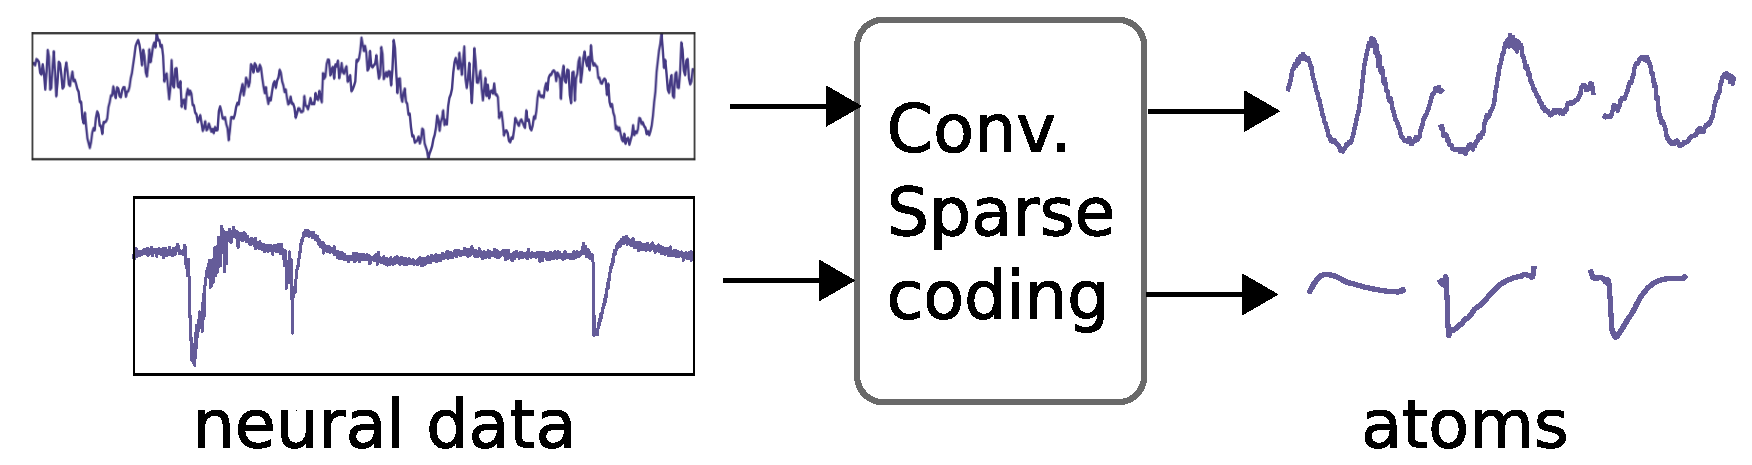
\includegraphics[width=0.85\linewidth]{figures/schema.pdf}
\end{center}
   \caption[]{Une illustration de la façon dont le codage à faible densité convolutionnelle peut être utilisé pour extraire automatiquement les formes d'onde prototypiques.}
   \label{fig:sommaire:csc_schematic}
\end{figure}

Cependant, les photos sont intrinsèquement différentes des données neuronales. Premièrement, les données neuronales peuvent être enfouies dans le bruit et corrompues par des artefacts de grande amplitude. Deuxièmement, les images sont étiquetées en raison de données provenant de la foule comme dans le cas d'Imagenet~\citep{deng2009imagenet}, mais les données neuronales ne le sont pas. Les annotations d'experts dans le cas de données neuronales ne sont pas facilement disponibles. Enfin, ce sont les données spatio-temporelles avec des dynamiques différentes du monde 3D que les photos capturent. 

C'est là que le codage convolutif à faible densité (CSC) peut jouer un rôle en extrayant des caractéristiques prototypiques des données, comme le montre la  Figure~\ref{fig:sommaire:csc_schematic}. Il s'agit d'un algorithme non supervisé de la vision par ordinateur, qui peut apprendre des dictionnaires de formes d'onde prototypiques (atomes) à partir des données en utilisant les opérations de convolution. Pour en savoir plus sur le CSC, le lecteur peut lire la Section~\ref{sec:background_dict_learning} de ce chapitre.

Les algorithmes CSC n'approximent pas le signal en utilisant la base de Fourier (ou sinusoïdale). Bien qu'il s'agisse de la technique conventionnelle d'extraction de signaux enfouis dans le bruit, l'approximation peut dégrader la forme du signal, ce qui peut être un biomarqueur dans de nombreuses maladies cliniques~\citep{cole2017brain}. . Par exemple, même avec un grand nombre de sinusoïdes de la base de Fourier, les bords d'une onde carrée ne peuvent pas être bien approximés. En effet, l'approximation imparfaite autour de ces bords est ce qu'on appelle souvent des artefacts d’oscillations parasites dans les contextes de traitement du signal. Bien sûr, les transitoires peuvent être mieux approximés en utilisant des ondelettes, mais ce n'est clairement pas suffisant pour d'autres formes de données. Plutôt que de fixer la base à Fourier ou à ondelettes, l'approche CSC consiste à apprendre à la fois la base et les coefficients.

Dans notre travail présenté au Chapitre~\ref{chapter:alphacsc},  nous étendons les algorithmes CSC conventionnels pour les bruits de queue lourds. Nous reformulons le problème d'optimisation sous forme d'inférence MAP avec une distribution “alpha-stable” pour remplacer la perte de reconstruction. Nos résultats montrent que ce type d'algorithme est robuste à la présence d'artefacts et peut être utilisé pour découvrir des structures temporelles à partir de signaux neuronaux, même ceux qui impliquent des oscillations imbriquées.

\section*{Chapitre~\ref{chapter:bids}: Brain Imaging Data Structure (BIDS)}

\begin{figure}[htb!]
\begin{center}
   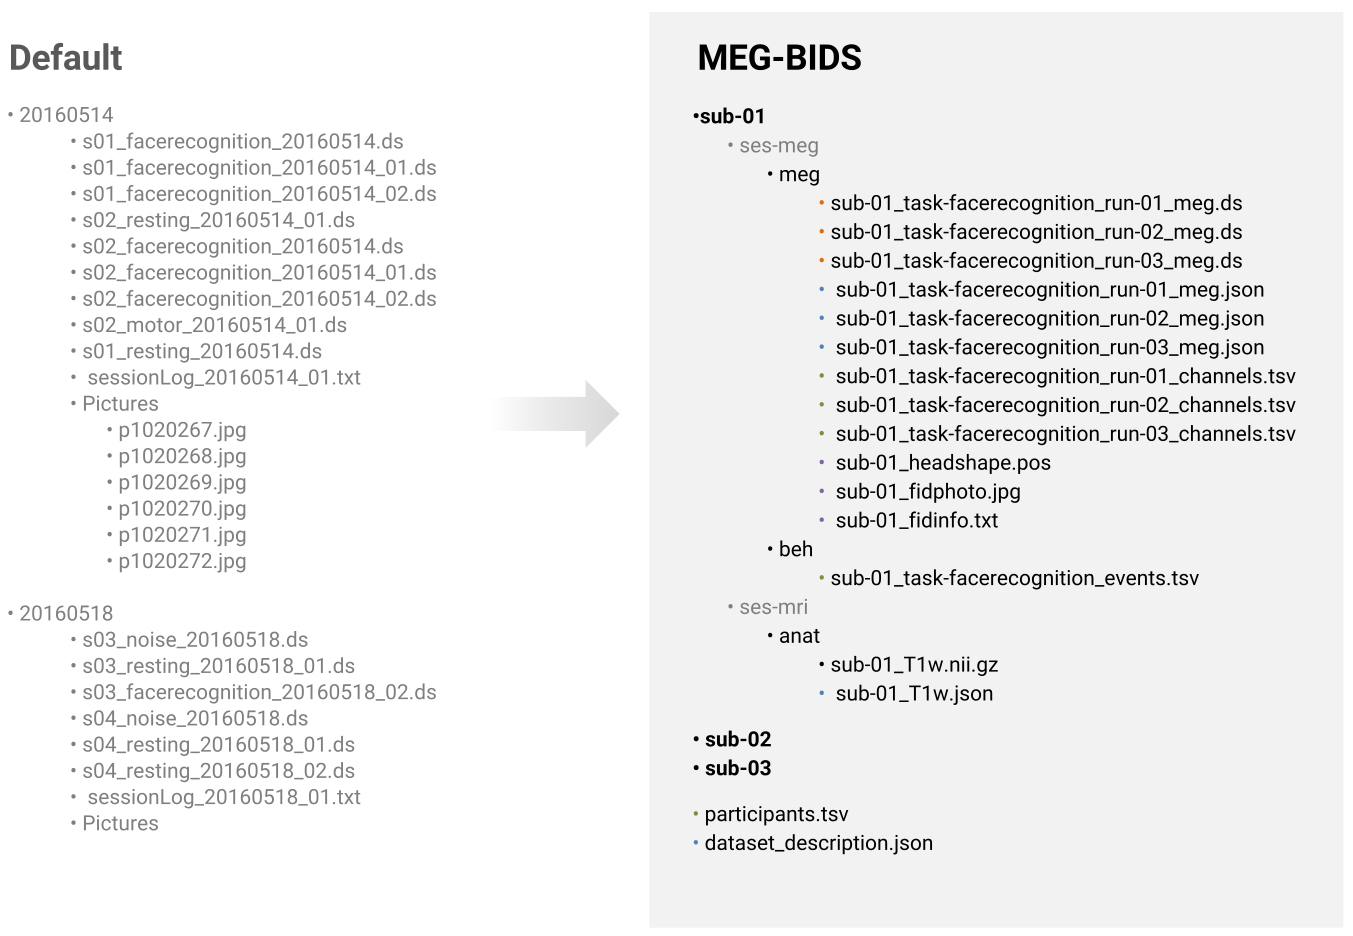
\includegraphics[width=\linewidth]{figures/bids_organization.png}
\end{center}
   \caption[]{Schéma d'organisation des données BIDS-MEG : Gauche : un schéma typique d'organisation de données par défaut où les dossiers sont organisés par date de session et contiennent différentes exécutions pour un participant donné dans une étude. Droite: BIDS-MEG organise les données par étude, puis par participant (sujet), suivi de la modalité, puis des sessions et finalement des runs. Notez les fichiers latéraux qui sont présents à tous les niveaux de la hiérarchie des données et documentez facilement le contenu des métadonnées.}
   \label{fig:sommaire:BIDS-MEG-organization}
\end{figure}
Du point de vue de la reproductibilité, le partage de données est d'une importance capitale. Le code de partage en soi ne permet pas la reproductibilité si les données qui l'accompagnent ne sont pas disponibles et sont coûteuses à acquérir. La réanalyse d'un ensemble de données est cependant utile non seulement du point de vue de la reproductibilité, mais aussi pour découvrir de nouveaux effets qui étaient auparavant négligés. En même temps, plus les données sont partagées, plus la taille de nos échantillons sera grande, ce qui nous permettra de mener des études avec une plus grande puissance statistique. En effet, la faible puissance statistique est l'une des principales raisons de la crise de la reproductibilité.

Bien que le partage de données en neurosciences soit à la hausse, la quantité de données ré-utilisées est encore limitée. Par exemple, depuis la publication des données du projet Human Connectome Project (HCP)~\citep{larson2013adding} du MEG en 2013, il y a eu très peu de cas de réutilisation de ces données. Au moment de la rédaction de cette thèse, nous n'avions qu'un ou deux cas documentés~\citep{jas2017autoreject} de réutilisation des données HCP. Même dans ces cas, l'effort s'est surtout limité à reproduire les résultats plutôt que de tester de nouvelles hypothèses. Cela représente clairement un écart entre l'idéal et la pratique du partage de données.

% Clearly, sharing data is not a panacea as the tools, skills and resources to process such large datasets is currently missing in typical laboratories. Perhaps the most important roadblock is standardization of metadata.

Les expériences de neuroimagerie sont souvent compliquées et impliquent différentes tâches cognitives (auditives, visuelles, somatosensorielles, \emph{etc.}), différents paramètres d'acquisition (fréquence d'échantillonnage, nombre de capteurs et leur emplacement, dispositif de mesure, etc.) et des paramètres de population (sexe, âge, \emph{etc.}). Toutes ces métadonnées sont des informations nécessaires pour réanalyser avec succès les données. Malheureusement, dans le passé, il n'y a pas eu de consensus entre les différents laboratoires et fabricants industriels sur ce qui constitue des métadonnées utiles. Cela souligne la nécessité d'établir des normes. Bien qu'à première vue, cela peut sembler être de la paperasserie bureaucratique inutile, en fait, des normes existent dans presque tous les aspects de notre vie.


Outre les méta-informations qui sont stockées avec les données, les données elles-mêmes sont stockées dans l'un des 10 à 20 formats de fichiers différents et à différents stades de traitement. Bien que des efforts aient déjà été déployés pour normaliser les structures de données~\citep{gibson2009minimum, grewe2011bottom, stoewer2013singlefile, teeters2015neurodata, bigdely2016preparing}, il n'a pas été largement accepté. La conception d'une nouvelle norme est délicate car elle nécessite l'obtention d'un consensus communautaire. En même temps, elle doit trouver le juste équilibre entre la rigidité pour l'efficacité et la flexibilité pour s'adapter aux technologies futures.

Le format BIDS~\citep{gorgolewski2016brain} est en effet conçu en tenant compte de ces considérations. La norme comporte une hiérarchie de dossiers pour décrire la technologie d'imagerie utilisée, le nom du sujet et la date de l'expérience. A chaque niveau de hiérarchie, les fichiers sont accompagnés de fichiers “json” latéraux décrivant les métadonnées. Un fichier json est un fichier texte facile à analyser qui contient des paires de clés et de valeurs, de sorte qu'il a l'avantage d'être lisible par l'homme et par la machine en même temps. Ces fichiers suivent un principe d'héritage, c'est-à-dire qu'un champ décrit dans un fichier json à un niveau supérieur de la hiérarchie sera automatiquement propagé en aval. La spécification principale de BIDS est accompagnée de spécifications d'extension qui décrivent des aspects spécifiques pour décrire différentes modalités.

En même temps, la norme n'existe pas isolément. Le consortium BIDS fournit également un écosystème croissant d'outils pour convertir les ensembles de données dans un format compatible BIDS et pour valider les données afin qu'elles soient conformes à la norme.

Dans ce travail, nous avons présenté une extension significative de BIDS pour soutenir les aspects spécifiques des données MEG. Comme nous le savons, la MEG fournit une mesure directe de l'activité cérébrale avec une résolution temporelle en millisecondes et des capacités d'imagerie à source unique. Jusqu'à présent, BIDS a fourni une solution pour structurer l'organisation des données d'IRM. Malgré l'absence d'un format de données standard pour la MEG, BIDS-MEG est une solution de principe pour stocker, organiser et partager les volumes de données typiquement importants produits. Il s'appuie sur BIDS pour l'IRM et permet donc une organisation multimodale des données par construction. Ceci est particulièrement utile pour l'enregistrement anatomique et fonctionnel de l'imagerie source MEG avec l'IRM. Avec BIDS-MEG et une gamme croissante de logiciels adoptant la norme, la communauté MEG dispose d'une solution pour minimiser les frais généraux de conservation, réduire les erreurs de traitement des données et optimiser l'utilisation des ressources informatiques pour l'analyse des données. La norme comprend également des métadonnées bien définies pour faciliter les efforts futurs d'harmonisation et de partage de données, ainsi que des extensions à d'autres modalités de données électrophysiologiques.

\subsection*{Outils logiciels}
Dans le cadre de cet effort, j'ai participé aux discussions pour décider de la norme. En même temps, j'ai développé l'extension MEG du validateur BIDS. Développé en javascript à l'aide de “nodejs”, il peut être packagé pour fonctionner dans le navigateur (Google Chrome). Une version en ligne de commande est également fournie afin qu'elle puisse être utilisée dans l'analyse par script. Le validateur effectue plusieurs contrôles de santé mentale sur les ensembles de données pour s'assurer qu'ils sont compatibles avec BIDS. Cela comprend l'utilisation d'expressions régulières pour vérifier les noms de fichiers et de schémas de notation d'objets JavaScript (JSON) pour s'assurer que les fichiers de métadonnées sont normalisés par type de données.

Afin de faciliter l'adoption du format BIDS, j'ai également contribué au code Python qui est utilisé pour convertir les jeux de données existants en jeux de données compatibles BIDS. Le code peut être trouvé ici : \url{https://github.com/mne-tools/mne-bids}. 

Pour une description plus détaillée de la spécification BIDS-MEG, des exemples de données, des ressources et des commentaires, veuillez visiter le site \url{http://bids.neuroimaging.io}.

\section*{Chapitre~\ref{chapter:group_study}: A reproducible M/EEG group study}

ans la section précédente, nous avons discuté de la façon dont le partage des données peut être facilité à l'aide du BIDS pour la MEG permettant de se rapprocher de l'objectif de reproductibilité. Cependant, la reproductibilité n'est pas obtenue en partageant simplement plus de données dans l'espoir que cela résoudra tous les problèmes. Comme l'indique Baker \citet{baker20161}, l'une des meilleures solutions pour favoriser la reproductibilité scientifique n'est pas technique, mais éducative. C'est bien sûr vrai pour les statistiques, où il y a un besoin urgent de clarifier et d'éduquer les chercheurs ces outils requis en neurosciences. Cela devient maintenant tout aussi important pour les logiciels académiques.

Au cours des dernières années, les boîtes à outils universitaires gratuites ont pris de plus en plus d'importance dans l'analyse du MEG pour diffuser des méthodes de pointe, partager les meilleures pratiques entre différents groupes de recherche et de mettre en commun des ressources pour développer des outils essentiels pour la communauté du MEG. Des événements pédagogiques sont régulièrement organisés dans le monde entier où les bases de chaque boîte à outils sont expliquées par ses développeurs et des utilisateurs expérimentés. Il y a toutefois des lacunes dans les connaissances qui doivent être comblées. Premièrement, la plupart des exemples d'enseignement ne montrent que l'analyse d'un seul ‘participant typique’, alors que la plupart des études réelles de MEG impliquent l'analyse de données de groupe. Il revient ensuite aux chercheurs sur le terrain de déterminer eux-mêmes comment faire la transition et obtenir des résultats significatifs pour le groupe. Deuxièmement, nous ne connaissons pas d'exemples d'analyse complète d'un même ensemble de données de groupe avec différentes boîtes à outils académiques pour évaluer le degré d'accord dans les conclusions scientifiques et comparer les forces et les faiblesses des diverses méthodes d'analyse et de leur mise en œuvre indépendante.

\section*{Les méthodes}
Pour répondre à cette question, un atelier a été organisé par les principaux développeurs des six boîtes à outils MEG les plus populaires à Biomag 2017. Ce travail fait suite à l'atelier, qui présente la contribution de l'équipe du logiciel MNE, et sera publié dans \emph{Frontiers in Neuroscience, section Brain Imaging Methods}. Cette étude présente les résultats obtenus par la réanalyse d'un ensemble de données ouvertes de \citet{wakeman2015multi} à l'aide du progiciel MNE. L'analyse couvre les étapes de prétraitement, l'assurance qualité, l'analyse de l'espace capteur des réponses évoquées, la localisation de source et les statistiques dans l'espace capteur et l'espace source. Les résultats avec les stratégies alternatives possibles sont présentés et discutés à différentes étapes telles que l'utilisation du filtrage passe-haut par rapport à la correction de base, le tSSS par rapport à la séparation spatiale du signal (SSS), l'utilisation d'une norme minimale inverse par rapport à la variance minimale linéairement contrainte (LCMV), et l'utilisation de statistiques univariées ou multivariées.

\section*{Résultats}

L'objectif est de fournir une étude comparative des différentes étapes du pipeline d'analyse MEG/EEG sur le même ensemble de données, avec un accès ouvert (\url{https://github.com/mne-tools/mne-biomag-group-demo}) to all of the scripts necessary to reproduce this analysis. An example of such a reanalysis figure is shown in Figure~\ref{fig:sommaire:grand_average} qui montre la réponse évoquée pour un capteur EEG. En effet, nous sommes en mesure non seulement de reproduire les résultats de \citet{wakeman2015multi}, mais aussi de mettre en évidence les facteurs qui pourraient conduire à des résultats différents. Le travail se termine par un ensemble de recommandations basées sur les leçons que nous avons tirées de cet exercice de réanalyse.

\begin{figure}[htb]
  \centering
  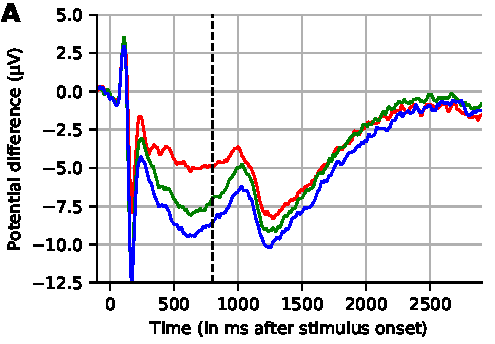
\includegraphics[width=0.7\linewidth]{figures/grand_average_highpass-NoneHz.pdf}\\
  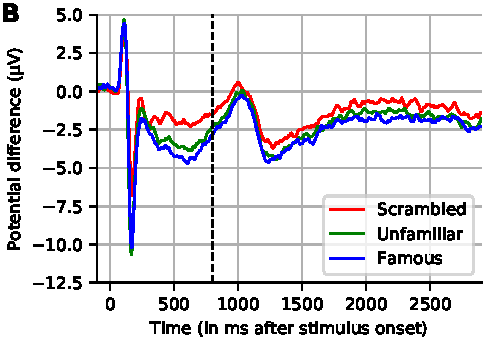
\includegraphics[width=0.7\linewidth]{figures/grand_average_highpass-1Hz.pdf}
\caption[]{Moyenne générale des réponses évoquées sur 16 sujets pour le canal EEG065. (A) Pas de filtre passe-haut. (B) Filtré passe-haut à 1,0 Hz. Il est à noter que, comme (A), les résultats rapportés par \cite{wakeman2015multi} (la ligne en pointillés à 800 ms indique où leur placette s'est arrêtée) montrent de grandes dérives, mais celles-ci reviennent à des niveaux proches de la ligne de base vers la fin d'un intervalle suffisamment long (ici, 2,9 secondes) même sans appliquer un filtre passe-haut.}
\label{fig:sommaire:grand_average}
\end{figure}  

\clearpage

\section*{Chapitre~\ref{chapter:autoreject}: Rejet automatisé des artefacts pour M/EEG}

Dans la section précédente, nous avons discuté des problèmes de reproductibilité lors de la réalisation d'études de groupe en MEG et EEG. L'automatisation est un moyen d'améliorer la reproductibilité. et nous avons brièvement évoqué un algorithme permettant d’automatiser la détection de segments de données incorrects, appelé \emph{autoreject}.

%copy pasted abstract below
Dans cette section, nous allons présenter cet algorithme qui rejette et répare les mauvais essais dans les signaux MEG et EEG. L'annotation de mauvais segments dans les données est peut-être l'un des aspects les plus chronophages du traitement de données électrophysiologiques. Actuellement, il est fait soit manuellement, soit en utilisant des algorithmes automatisés mais qui présentent l’inconvénient d’être des boîtes noires (par exemple, RANSAC~\citep{bigdely2015prep}, FASTER~\citep{nolan2010faster}, SNS~\citep{de2008sensor}). L'approche manuelle est souvent subjective et sans consensus clair notamment sur ce qui compose un segment de données corrompu. Par conséquent, la réanalyse est non seulement exigeante manuellement, mais peut également entraîner des problèmes de reproductibilité. En revanche, les méthodes automatisées sont contrôlées par des paramètres difficiles à régler. En cas d'échec, il n'est pas toujours évident de savoir ce qui a causé l'échec de la méthode et comment elle a pu être corrigée. Par conséquent, il n’y a pas d'autre choix que d'exclure les données de l'analyse ultérieure.

\subsection*{Les méthodes}

\begin{figure}[htb]
	\centering
	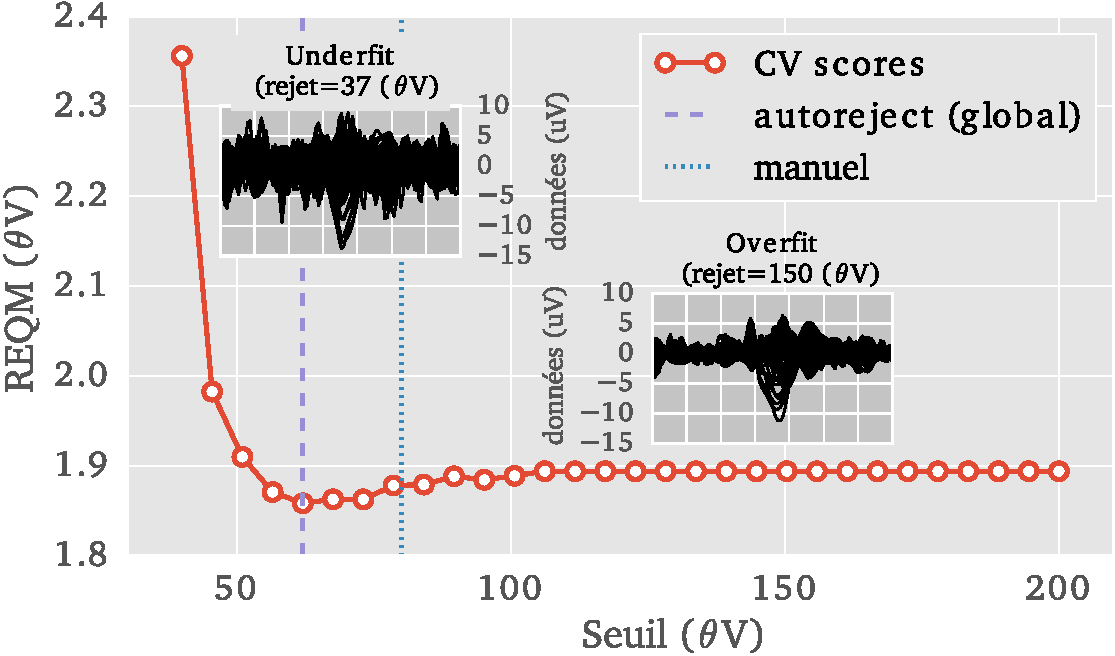
\includegraphics[width=0.8\linewidth]{figures/figure1_sommaire.pdf}
    \caption[]{Erreur de validation croisée en fonction du seuil de rejet crête à crête sur un ensemble de données EEG. Le racine de l'erreur quadratique moyenne (REQM) entre la moyenne de l'ensemble de formation (après avoir retiré les essais marqués comme étant mauvais) et la médiane de l'ensemble de validation a été utilisée comme mesure de validation croisée (Section~\ref{sec:auto_global}). Les deux cartons montrent la moyenne des essais sous forme de ``parcelles papillon" (chaque courbe représentant un capteur) respectivement pour des seuils très bas et élevés. Pour les seuils bas, le REQM est élevé parce que la plupart des essais sont rejetés (\emph{underfit}). Pour des seuils élevés, le modèle n'abandonne aucun essai (\emph{overfit}). Le seuil optimal basé sur les données \emph{(autoreject, global)} avec un minimum de REQM se situe quelque part entre les deux. Il correspond approximativement au seuil humain.}
    \label{fig:sommaire:cross_val}
\end{figure}

Cela nous a conduit à développer une méthode basée sur des choix de conception motivés par la facilité d’interprétation et de diagnostic. La méthode que nous proposons capitalise sur la validation croisée (Figure~\ref{fig:sommaire:cross_val}) en conjonction avec une métrique d'évaluation robuste pour estimer le seuil optimal pic à pic, une quantité couramment utilisée pour identifier les mauvais essais en MEG / EEG. L'idée clé est que les ensembles de formation et de validation sont d’autant plus similaires lorsque les données ne contiennent pas de valeurs aberrantes. Ainsi, un seuil qui minimise l'erreur de validation croisée est un seuil qui supprime les valeurs aberrantes. En effet, comme le montre la Figure~\ref{fig:sommaire:cross_val}, pour des seuils très bas, trop d'essais sont supprimés, ce qui se traduit par une moyenne bruitée, alors que pour des seuils très élevés, les valeurs aberrantes ne sont pas éliminées. L’optimum se situe entre les deux, ce qui peut être estimé en minimisant l’erreur de validation croisée.

Cette approche est ensuite étendue à un algorithme plus sophistiqué qui estime ce seuil au niveau des capteurs. Il en résulte une liste des mauvais capteurs par essais. En fonction du nombre de capteurs défectueux, l'essai est ensuite corrigé par interpolation ou exclue de l'analyse. Pour des raisons d'efficacité, nous utilisons l'optimisation bayésienne, technique bien connue pour l'optimisation hyperparamétrique. Toutes les étapes de l'algorithme sont entièrement automatisées, d’où le nom \emph{autoreject}. Il est important de noter que l'algorithme est même capable de traiter des capteurs qui sont localement corrompus, ce qui est souvent le cas pour les données EEG.


\subsection*{Résultats}

\begin{figure}[htb]
    \centering
    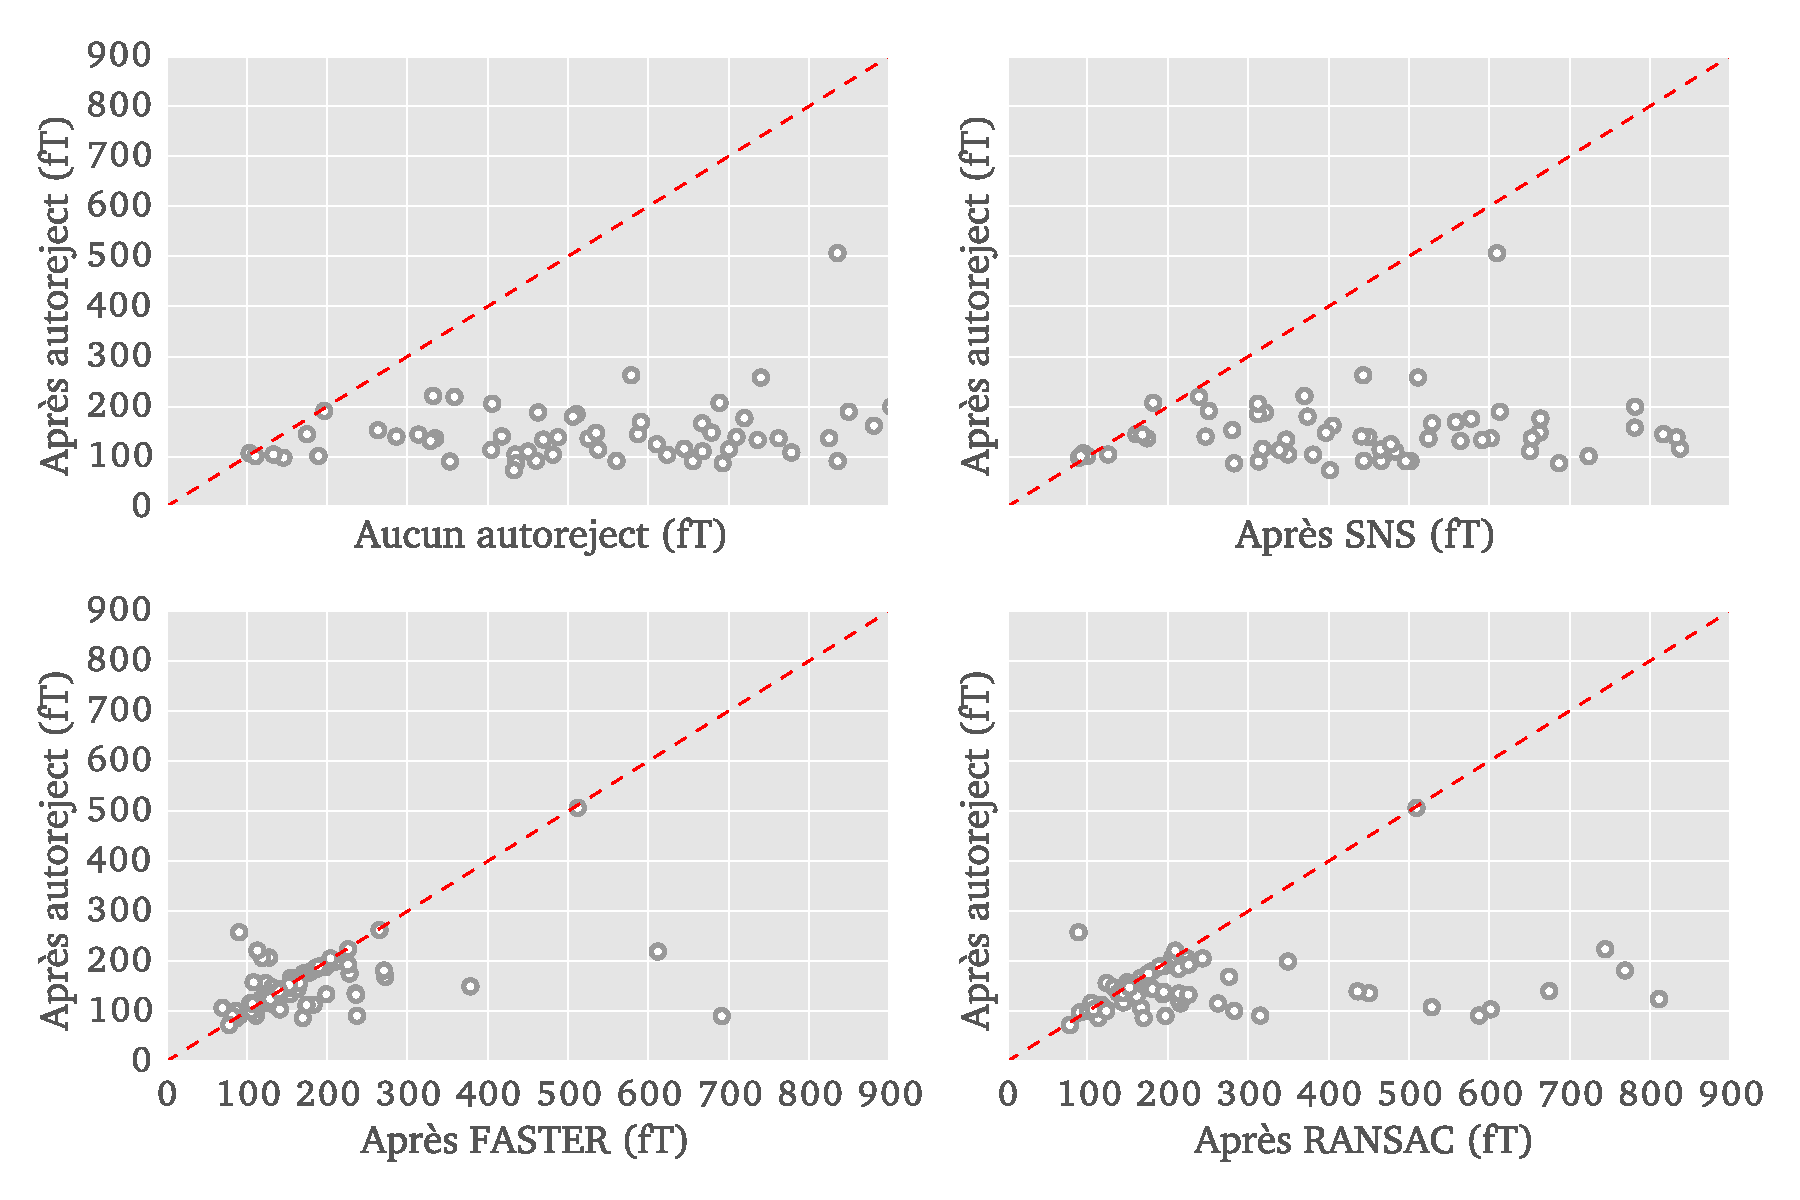
\includegraphics[width=\linewidth]{figures/figure4_sommaire.pdf}
    \caption[]{Diagrammes de dispersion pour les résultats avec les données HCP. Pour chaque méthode, on utilise la norme $\infnorm{\cdot}$ de la différence entre la vérité terrain HCP et la méthode. Chaque cercle représente un sujet. (A) \textit{autoreject (local)} \emph{vs.} aucun rejet, (B) \textit{autoreject (local)} \emph{vs.} Sensor Noise Suppression (SNS) (SNS), (C) \textit{autoreject} \emph{vs.} FASTER, (D) \textit{autoreject (local)} \emph{vs.} RANSAC. Les points de données sous la ligne rouge pointillée indiquent les sujets pour lesquels l'\textit{autoreject (local)} surpasse la méthode alternative.}
    \label{fig:sommaire:hcp_scatter}
\end{figure}

\begin{figure}[htb!]
	\centering
	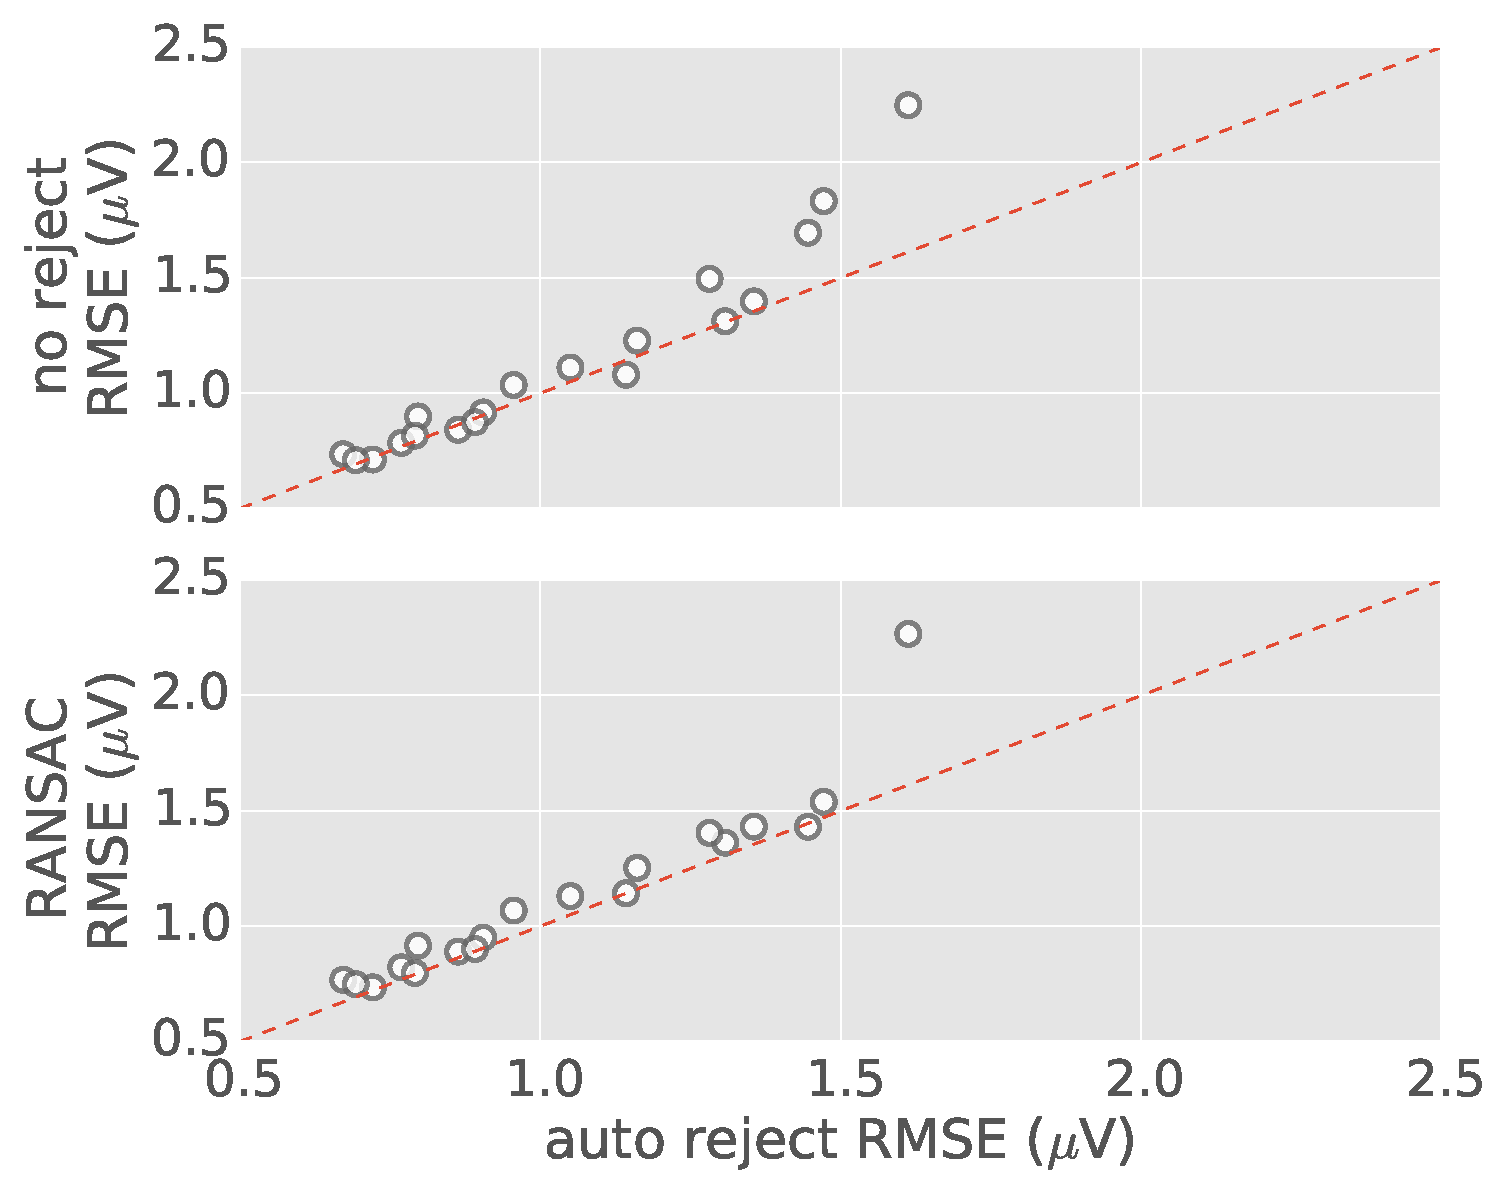
\includegraphics[width=0.9\linewidth]{figures/figure5.pdf}
    \caption[]{La réponse évoquée (moyenne des données d'un essai à l'autre) sur trois ensembles de données différents avant et après l'application de l'\emph{autoreject} --- es données de l'échantillon MNE, les données HCP et les données EEG Faces. Chaque capteur est une ligne sur les tracés. A gauche, les mauvais capteurs annotés manuellement sont affichés en rouge. L'algorithme trouve automatiquement les mauvais capteurs et les corrige pour les essais en question. A noter que l’algorithme peut également corriger plusieurs capteurs à la fois et fonctionne pour tout type de modalités d'acquisition.}
    \label{fig:sommaire:sample_evoked}
\end{figure}

Afin d'évaluer l'importance pratique de l'algorithme, nous avons effectué une validation approfondie et des comparaisons avec des méthodes de pointe sur quatre ensembles de données publiques contenant des enregistrements MEG et EEG de plus de 200 sujets. Les comparaisons comprennent des efforts purement qualitatifs (Figure~\ref{fig:sommaire:sample_evoked}) ainsi que des analyses comparatives quantitatives par rapport à des pipelines de prétraitement sous surveillance humaine (Figure~\ref{fig:sommaire:hcp_scatter}) et semi-automatique. Nos comparaisons qualitatives ont montré qu'\emph{autoreject} était capable d'annoter et de réparer les segments défectueux de manière satisfaisante pour ces différents ensembles de données. En effet, l'algorithme permet d'automatiser le prétraitement des données MEG depuis le HCP jusqu'au calcul des réponses évoquées. La nature automatisée de notre méthode minimise le fardeau de l'inspection humaine, ce qui favorise l'extensibilité et la fiabilité exigées par l'analyse des données dans les neurosciences modernes.

\section*{Chapitre~\ref{chapter:alphacsc}: Temporal representation learning}

Jusqu'à présent, nous avons étudié l'automatisation en neuroimagerie dans le but de permettre une analyse évolutive des données, ainsi qu’une reproductibilité. Malgré le fait que la reproductibilité et l'analyse de données à grande échelle nous permettent de consolider les études existantes, elles ne sont pas en soi des outils faits pour découvrir des phénomènes nouveaux et intéressants. Dans cette section, nous explorerons cette dimension de l'automatisation à l'aide de ce qu'on appelle \emph{l'apprentissage de la représentation}.

Les représentations sont les bases du traitement de signal. Il est assez facile de se convaincre de ce fait, si nous utilisons simplement une Transformée de Fourier Rapide (TFR) pour filtrer les données. Lorsque nous utilisons une TFR, nous sommes effectivement en train de décomposer le signal en une somme de sinusoïdes de fréquences variables. Si nous sommes intéressés par une analyse temps-fréquence, un choix commun de représentation pour des signaux en neuroscience consiste en l’utilisation des ondelettes de Morlet.

Traditionnellement, le choix de la représentation était principalement motivé par la préoccupation analytique et la facilité de la manipulation mathématique. Toutefois, l'essor récent de l'apprentissage profond a suscité un intérêt pour les représentations axées sur des données. C'est parce que de bonnes représentations qui capturent de manière compacte les propriétés des données sont essentielles pour des systèmes d'apprentissage efficaces et précis. Par exemple, en vision par ordinateur, les attributs artisanals telles que les descripteurs SIFT~\citep{lowe1999object} et GIST~\citep{oliva2001modeling}, Deformable Parts Model (DPM)~\citep{felzenszwalb2010object}, Histogram of Oriented Gradient (HOG)~\citep{dalal2005histograms} \emph{etc.} étaient la norme, avant qu’on ne réalise que l'apprentissage non supervisé et les auto-encodeurs performent bien mieux.

Aujourd'hui, l'apprentissage non supervisé est utilisé comme première étape dans une tâche d'apprentissage supervisé en vision par ordinateur. L'apprentissage de la représentation, en soi, n'est peut-être pas aussi intéressant, hormis pour les visualisations diagnostiques en apprentissage profond~\citep{zeiler2014visualizing}. Malgré cela, il y a toujours eu un intérêt à comprendre les représentations dans le cerveau humain (en particulier le système visuel), puisqu’il était pensé que cela nous aiderait à construire de meilleurs systèmes d'apprentissage. L'un des pionniers dans ce domaine de recherche est Bruno Olshausen, dont les travaux sur l'apprentissage de dictionnaire~\citep{olshausen1996emergence}ont démontré que les patches de Gabor sont effectivement fondamentaux pour les images naturelles, similaires à ceux que Hubel et Wiesel~\citep{hubel1962receptive, marcelja1980mathematical} ont trouvés dans le cortex visuel du chat, et à ce qui est utilisé dans les caractéristiques de GIST. Hormis ces études, la représentation apprise en elle-même n'est pas considérée comme aussi significative que les mesures de performance comme le score de prédiction ou la perte de reconstruction. Cependant, lorsqu’il s’agit de signaux neuronaux, nous avons réalisé que ce n'est pas le cas et que la fidélité de la représentation est en soi intéressante. En effet, la forme du signal est un biomarqueur crucial dans de nombreuses applications cliniques des neurosciences~\citep{cole2017brain}. 

Un développement parallèle dans le domaine de la neuroimagerie a été la hausse d’intérêt pour l'apprentissage de formes prototypiques qui sont shift-invariantes~\citep{jost2006motif, barthelemy2013multivariate, brockmeier2016learning, hitziger2017adaptive}. Elle est motivée par le fait que les approximations existantes utilisant la base de Fourier déforment souvent le signal. Il y a, par exemple, un débat au niveau du type de filtre qui devrait être utilisé (voir Section~\ref{sec:group_study_temporal_filtering} et \cite{widmann2015digital,parks1987digital,ifeachor2002digital, gotz-etal:15}). 
Même s’il y a certains succès qui ont été rapportés en neuroimagerie avec ces algorithmes, leur applicabilité est limitée en raison de leur nature heuristique. Étonnement, jusqu'à présent, il y a eu très peu de pollinisation croisée d'idées entre les communautés de vision par ordinateur et de neuroimagerie sur ces aspects. Notre travail est une tentative de combler cette lacune. Nous proposons un modèle qui s'appuie sur les creuses modèles de codage shift-invariants existants, de manière à pouvoir traiter les bruits de queue lourds et les artefacts. Il suppose la positivité des coefficients, pour tenir compte du fait qu'un atome ne change pas de polarité à travers le temps.

\subsection*{Les méthodes}

\begin{figure}[htb]
    \centering
     \subfigure[$K=10$, $L=32$.]{
     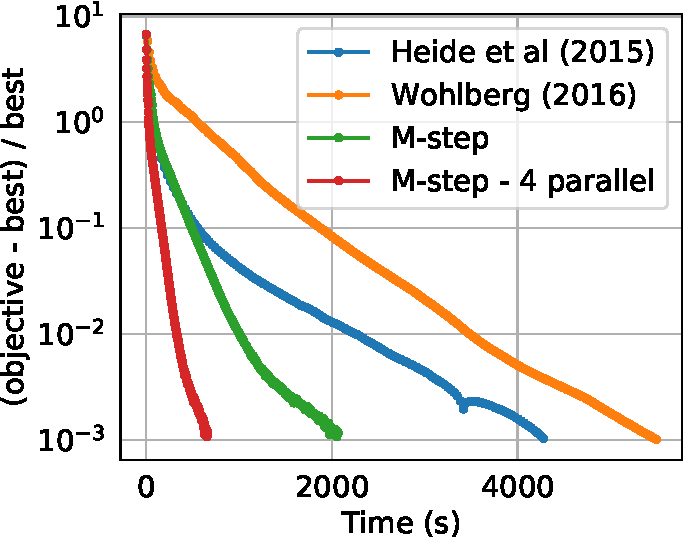
\includegraphics[width=0.5\linewidth]{figures/relative_10_32.pdf}} \\
     \subfigure[Temps nécessaire pour atteindre une précision relative de 0.01.]{
     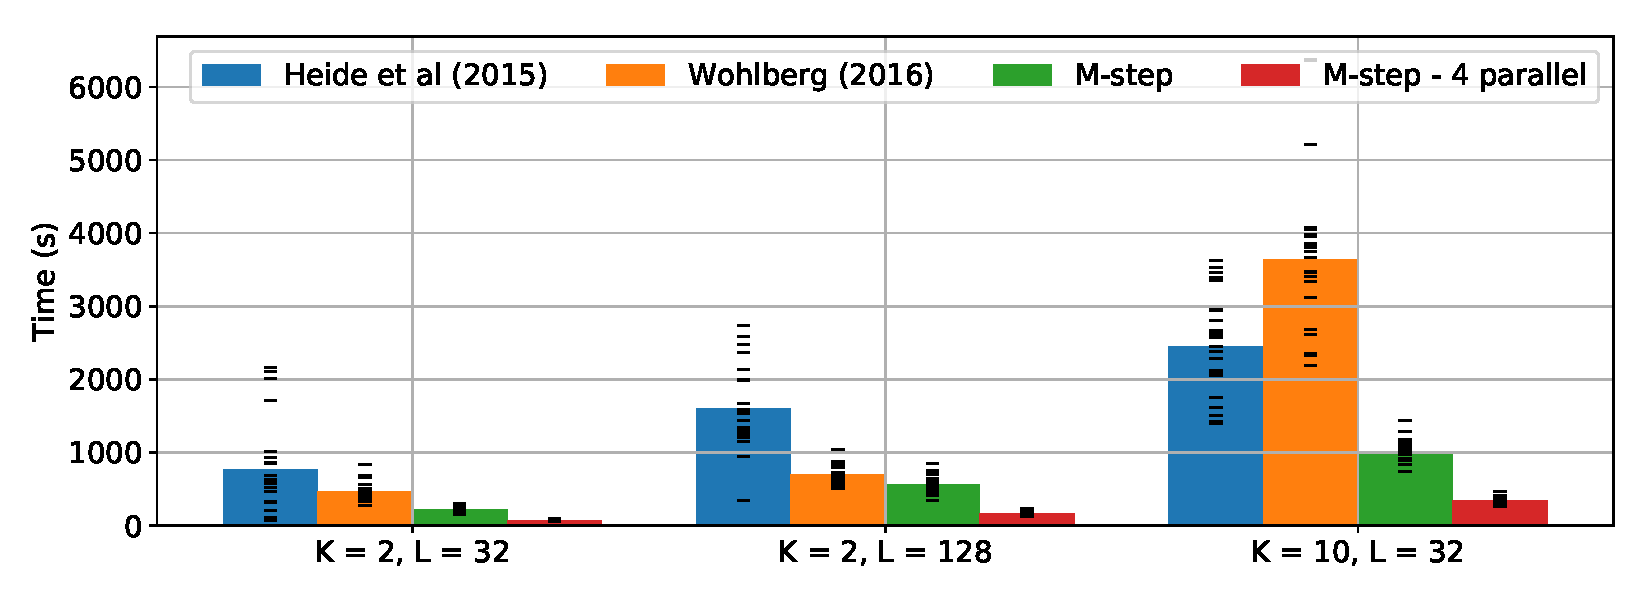
\includegraphics[width=\textwidth]{figures/bar_plot.pdf}}
    \caption[]{~Comparaison des méthodes de pointe avec notre approche. (a)~Diagramme de convergence avec la fonction objectif par rapport au minimum obtenu, en fonction du temps de calcul. (b)~Temps nécessaire pour atteindre une précision relative de $10^{-2}$, pour différents réglages du nombre d'atomes $K$ et de la longueur d'un atome $L$.}
    \label{fig:sommaire:convergence}
\end{figure}

Un modèle CSC, tel qu'introduit pour la première fois par \citet{grosse2012shift}, exprime le signal estimé $\hat{x}_n$ comme une somme de convolution des atomes $d^k$  et de leurs activations correspondantes $z_n^k$:

\begin{align}
z_{n,t}^k \sim {\cal E}(\lambda),
\quad x_{n,t} | z, d \sim {\cal N}( \hat{x}_{n,t},1 ),
\quad \text{ where,}
\quad \hat{x}_n \triangleq \sum_{k=1}^{K}d^{k} * z_{n}^{k} \enspace .
\label{eqn:sommaire:csc_prob}
\end{align}

Dans le modèle traditionnel, le bruit est supposé être de distribution gaussienne $\cal N(\cdot)$ et les activations sont supposées être creuse, tirées d'une distribution exponentielle $\cal E(\cdot)$. Les activations et les atomes sont estimés à l'aide d'un autre schéma de minimisation. Le modèle que nous présentons est un nouveau modèle probabiliste du CSC pour l'apprentissage d'atomes shift-invariants, à partir de données de séries temporelles neuronales non traitées contenant des artefacts potentiellement importants. Par conséquent, un modèle de bruit gaussien n'est plus suffisant. Au cœur de notre modèle, que nous appelons $\alpha$CSC, se trouve une famille de distributions à queue lourdes appelées $\alpha$-stable distributions. Le paramètre $\alpha$ contrôle la lourdeur de la distribution.

Nous développons un algorithme nouveau et efficace sur le plan informatique, pour la maximisation de l'espérance de Monte Carlo (MCEM), pour l'inférence. L'étape de maximisation se résume à un problème CSC pondéré (Equation~\ref{eq:sommaire:problem_definition_z}), pour lequel nous développons un algorithme d'optimisation efficace.

\begin{align}
- & \max_{z, d} \sum_{n=1}^{N} \Big( \|\sqrt{w_{n}} \odot (x_{n} - \sum_{k=1}^{K}d^{k} * z_{n}^{k})\|_{2}^{2} + \lambda \sum_{k}{ \|{z}_{n}^{k} \|_1}\Big) \quad \text{ s.t.  } {z}_n^k \geq 0, \forall n,k\enspace .
\label{eq:sommaire:problem_definition_z}
\end{align} 

Les poids $w_n$ dans l'étape de maximisation sont estimés dans l'étape d'attente par l’usage d'une procédure de Monte Carlo à chaîne de Markov (MCMC). En effet, les poids nous aident à traiter les artefacts en les supprimant dans la fonction d'objectif de l'étape de maximisation.

\section*{Résultats}
\begin{figure}[htb]
    \centering
             \subfigure[LFP spike data from \cite{hitziger2017adaptive}]{
             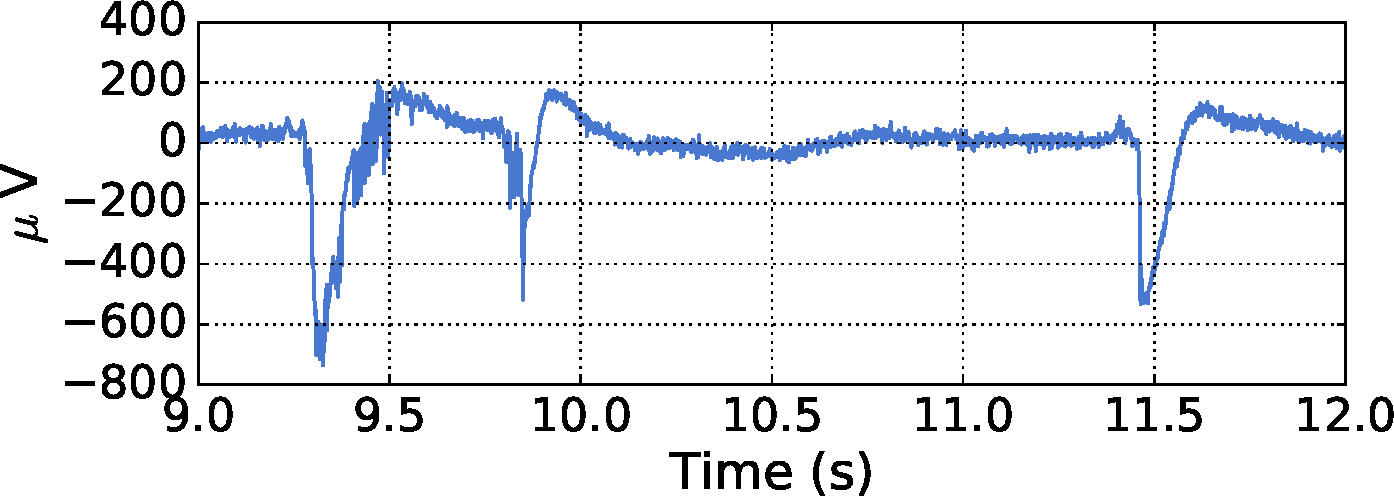
\includegraphics[height=4cm]{figures/spike_atomsa.pdf}
             } \\
             \subfigure[Estimated atoms]{
             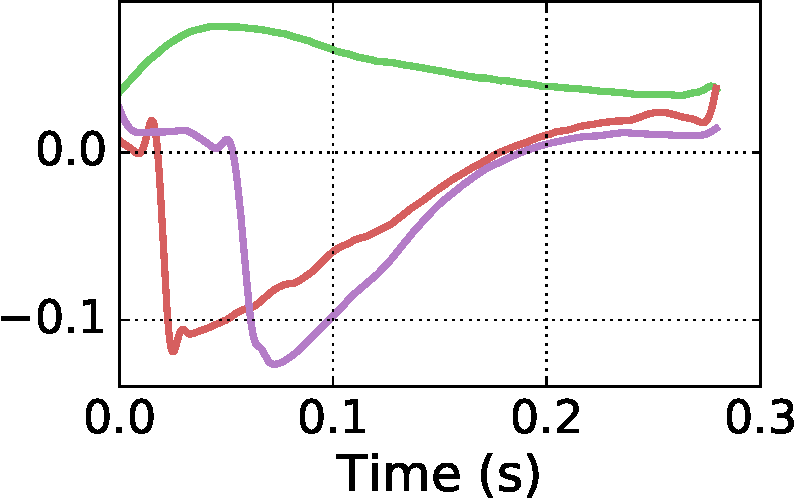
\includegraphics[height=4cm]{figures/spike_atomsb.pdf}
             }

            \caption[]{Atomes appris par $\alpha$CSC sur les données LFP contenant des pointes épileptiformes avec $\alpha=2$.}
            \label{fig:sommaire:spikedata}
\end{figure}

Dans notre travail, nous évaluons rigoureusement l'efficacité informatique de notre algorithme par rapport aux benchmarks concurrents. Parce que le problème CSC est non convexe, la procédure d'optimisation implique des boucles imbriquées et l'analyse théorique est souvent insuffisante pour traiter la complexité des fonctions non convexes. La procédure d'optimisation est imbriquée car le problème est convexe lorsque l'une des variables est fixe : les atomes ou les activations. La boucle extérieure alterne entre ces deux variables, tandis que la boucle intérieure les apprend lorsque l'autre est fixe. Le résultat final dépend de l'initialisation et, par conséquent, les algorithmes ne peuvent être comparés que s'ils sont testés pour de nombreuses initialisations aléatoires différentes et leurs résultats moyennés. Notre analyse qualitative va également au-delà du récit de la vérification de l'existence de formes d'onde connues pour découvrir des structures plus complexes dans les données.

Nos résultats démontrent que l'algorithme proposé atteint des vitesses de convergence de pointe (Figure~\ref{fig:sommaire:convergence}). En effet, notre algorithme utilise des solveurs quasi-Newton, ce qui permet une convergence plus rapide par rapport aux méthodes ADMM~\citep{heide2015fast, wohlberg2016efficient}. De plus,  $\alpha$CSC est significativement plus robuste aux artefacts, lorsqu’on le compare aux trois algorithmes concurrents : il peut extraire des \emph{spike bursts} (Figure~\ref{fig:sommaire:spikedata}), des oscillations, et même révéler des phénomènes plus subtils tels que le couplage de fréquences croisées lorsque appliqué à des séries temporelles neuronales bruyantes.

\section*{Conclusion}

La recherche en neuroimagerie est un mariage entre l'informatique et les neurosciences. Il s'agit d'une collaboration entre deux disciplines complémentaires -- le but est d'apporter à la table des outils de calcul qui peuvent aider les scientifiques à faire de nouvelles découvertes. Certains aspects de ce sous-domaine interdisciplinaire consistent bien sûr à développer progressivement les outils existants : par exemple, ceux qui peuvent aider à obtenir un meilleur score de prédiction ou une meilleure précision de localisation dans l'estimation des sources neuronales. Cependant, un aspect orthogonal mais tout aussi important de la recherche méthodologique est de développer des outils qui permettent à de nouvelles façons fondamentales d'interagir avec les données. Cette thèse est une tentative de faire avancer cet objectif en développant des outils pour l'analyse automatisée en électrophysiologie.

Il est devenu évident pour nous que, pour atteindre l'objectif d'une recherche reproductible, les grands ensembles de données publiques sont la clé et les méthodes automatisées pour les analyser sont indispensables. Alors que l'ambition de tout neuroscientifique est de générer de nouvelles connaissances et de pousser les frontières de notre connaissance du cerveau, cela n'est souvent pas possible en raison de la faible taille de l'effet dans de petits ensembles de données. Lorsque l'hypothèse nulle ne peut être rejetée, il est pratique courante de commencer partir à la recherche  de résultats significatifs en testant de multiples hypothèses et en rapportant les plus favorables. Cela a résulté en un corpus de littérature où une grande partie des résultats repose sur des bases incertaines.
 

Dans cette thèse, nous avons développé une nouvelle spécification connue sous le nom de BIDS, qui facilite le partage de données entre neuroscientifiques en promouvant des normes communes pour le stockage des métadonnées relatives aux mesures. Nous avons également donné un aperçu des défis que pose l'analyse de données reproductibles, en ce qui concerne les données MEG/EEG. En tant que contributeurs au progiciel MNE, nous nous sommes sentis particulièrement bien placés pour relever les défis liés aux logiciels : pipelines complexes, versions logicielles, initialisation aléatoire, etc. et recommandations normalisées pour chaque étape de ces pipelines. Pour ce faire, nous avons ré-analysé une étude de groupe sur l'ensemble de données Faces ~\citep{wakeman2015multi}.Pour assurer la reproductibilité des résultats, l'ensemble de l'analyse a été scriptée et les tracés ont été générés automatiquement à l'aide du logiciel \code{sphinx\_gallery}\footnote{https://sphinx-gallery.github.io}.

Afin de pousser encore plus loin l'objectif de reproductibilité via l'automatisation, nous avons développé deux nouvelles méthodes d'analyse des données électrophysiologiques. La première méthode, appelée \emph{autoreject}, vise à améliorer la suppression des segments de données contenant des artefacts, qui est une étape de prétraitement de base dans presque toutes les chaînes d'analyse. Nous développons une méthode efficace qui utilise une méthode de recherche de paramètres connue sous le nom d'optimisation bayésienne. Notre approche a été en mesure de faciliter la réanalyse des données du \ac{HCP} aux fins de l'analyse comparative. Notre deuxième méthode, connue sous le nom \emph{alphacsc}, permet d'extraire des séries temporelles neuronales pour de nouvelles structures oscillatoires. Non seulement cela, c'est un outil pour estimer des formes d'onde plus précises que ce qui est possible en utilisant l'analyse de Fourier traditionnelle. Dans notre travail, nous avons démontré qu'il était capable de découvrir des oscillations imbriquées à partir des données.

Ces technologies peuvent encore être considérées comme étant à leurs balbutiements à bien des égards. Tout comme les méthodes de localisation des sources dans le MEG/EEG ont évolué des modèles basés sur les dipôles vers des méthodes distribuées vers des modèles plus sophistiqués mettant en œuvre une esparsité structurée, ces nouvelles méthodes sont susceptibles de subir un processus évolutif d'améliorations incrémentielles. Si l'on considère l'exemple du CSC, notre modèle basé sur des distributions alpha-stables a étendu les modèles de vision par ordinateur de manière à pouvoir gérer des distributions à queue lourde, ce qui est caractéristique des données neuronales. Évidemment, ce n'est pas la fin du chemin. Ajuster les hyperparamètres dans les modèles CSC est encore notoirement difficile, mais ce n'est pas impossible s'il y a une tâche supervisée à la fin du pipeline. Les dictionnaires multi-échelles peuvent être critiques pour les signaux cérébraux, étant donné que les oscillations peuvent avoir un support variable. Comme le problème n'est pas convexe, des stratégies d'initialisation plus intelligentes comme celles basées sur MCMC pourraient conduire à des estimations plus précises~\citep{bachem2016fast}. Il sera bientôt nécessaire de construire des algorithmes CSC basés sur des approximations stochastiques, pour traiter de plus grands ensembles de données.

Contrairement à la vision par ordinateur ou au traitement du langage naturel, les industries à haut risque comme les soins de santé exigent des algorithmes transparents. Il ne suffit plus de se contenter d'une plus grande précision de prédiction. Dans nos travaux sur l'\emph{autoreject} et l'\emph{alphacsc}c, nous utilisons ces données publiques pour développer des algorithmes faciles à interpréter et à diagnostiquer. \emph{Autoreject} identifie les segments de données à supprimer sur la base d'un paramètre unique, facile à comprendre et réglé automatiquement. De la même manière, \emph{alphacsc} exploite directement les formes d'onde prototypiques, afin de remplacer les mesures indirectes pour mettre au jour des phénomènes d'intérêt.

Dans cette thèse, j'ai décrit une stratégie pour une recherche reproductible dans le futur : des ensembles de données publiques avec des échantillons de grande taille et de l'automatisation. Cependant, certains de mes travaux se sont limités à l'automatisation à l'échelle d'un seul sujet. Même si cela nous permet d'analyser de grands ensembles de données, cela peut parfois être limitatif, puisque ca ne nous permet pas de mettre en commun les données entre les sujets, de manière à pouvoir découvrir des effets plus subtils. Alors que nous entrons dans une ère de science rapide, de tels outils basés sur les données deviendront indispensables. Bien qu'un grand nombre de méthodes de recherche aient été axées sur l'amélioration du rapport signal/bruit dans chaque ensemble de données, cela peut s'avérer moins important lorsqu'il s'agit de traiter d'ensembles de données plus importants. Pour l'avenir, nous préférerons de plus en plus de grands ensembles de données qui ne sont pas parfaitement débruités, plutôt qu'un plus petit ensemble de données parfaitement débruité. De nouveaux outils devront être développés afin de permettre aux cliniciens de sonder rapidement le cerveau, de manière à identifier les signaux et les structures d'intérêt, de quantifier les incertitudes ainsi que les scores de précision, d'effectuer des contrôles de qualité et de visualiser interactivement leurs données.

